%!TEX root = edance.tex
%%%%%%%%%%%%%%%%
%   CHAPTER 6  %
%%%%%%%%%%%%%%%%
\chapter{PN Junction Currents}
\label{ch:ch06_pn_currents}
\graphicspath{{./figs_pn_currents/}}
%%%%%%%%%%%%%%%%%%%%%%%%%%%%%%%%%%%%%%%%%%%%%%%%%%%%%%%%%%%%%%%%%%%%%%%%%%%%%%%%%%%%%%%%
%%%%%%%%%%%%%%%%%%%%%%%%%%%%%%%%%%%%%%%%%%%%%%%%%%%%%%%%%%%%%%%%%%%%%%%%%%%%%%%%%%%%%%%%
%                                   SECTION 6.1                                        %
%%%%%%%%%%%%%%%%%%%%%%%%%%%%%%%%%%%%%%%%%%%%%%%%%%%%%%%%%%%%%%%%%%%%%%%%%%%%%%%%%%%%%%%%
%%%%%%%%%%%%%%%%%%%%%%%%%%%%%%%%%%%%%%%%%%%%%%%%%%%%%%%%%%%%%%%%%%%%%%%%%%%%%%%%%%%%%%%%
\section{Chapter Preview}
This chapter is a continuation of the previous chapter and builds on the knowledge that you've gained with regards to pn junctions.  The main focus is to derive the current-voltage ($I-V$) relations  for a diode.  We will demonstrate that diodes are ``one way streets" allowing current to flow in one direction (from p to n), but essentially shut off and behave as open circuits when current flows in the other direction.  To derive the $I-V$ curve, we need to cover a lot of preliminary material, such as the carrier concentration in non-equilibrium, in other words when $n p \neq n_i^2$.  We will use the current continuity equation to investigate how minority carriers diffuse across a region of majority carriers, and find that the diode $I-V$ curve is essentially determined by how minority carriers behave as they are injected into the p and n regions.  Finally, in the last part of this chapter, we'll investigate photovoltaic cells, or simply solar cells, and light-emitting diodes (LEDs), two important applications of $PN$-junctions.
%%%%%%%%%%%%%%%%%%%%%%%%%%%%%%%%%%%%%%%%%%%%%%%%%%%%%%%%%%%%%%%%%%%%%%%%%%%%%%%%%%%%%%%%
%%%%%%%%%%%%%%%%%%%%%%%%%%%%%%%%%%%%%%%%%%%%%%%%%%%%%%%%%%%%%%%%%%%%%%%%%%%%%%%%%%%%%%%%
%                                   SECTION 6.2                                        %
%%%%%%%%%%%%%%%%%%%%%%%%%%%%%%%%%%%%%%%%%%%%%%%%%%%%%%%%%%%%%%%%%%%%%%%%%%%%%%%%%%%%%%%%
%%%%%%%%%%%%%%%%%%%%%%%%%%%%%%%%%%%%%%%%%%%%%%%%%%%%%%%%%%%%%%%%%%%%%%%%%%%%%%%%%%%%%%%%
\section{Qualitative Overview of Diode Currents}
%%%%%%%%%%%%%%%%%%%%%%%%%%%%%%%%%%%%%%%%%%%%
%             SUBSECTION 6.2.1             %
%%%%%%%%%%%%%%%%%%%%%%%%%%%%%%%%%%%%%%%%%%%%
\subsection{Diode under Thermal Equilibrium}
%%%%%%%%%%%%%%%%%%%%%%%%%%%%%%%%%%%%%%%%%%%%
%                 FIGURE                   %
%%%%%%%%%%%%%%%%%%%%%%%%%%%%%%%%%%%%%%%%%%%%
\begin{figure}[tb]
\centering
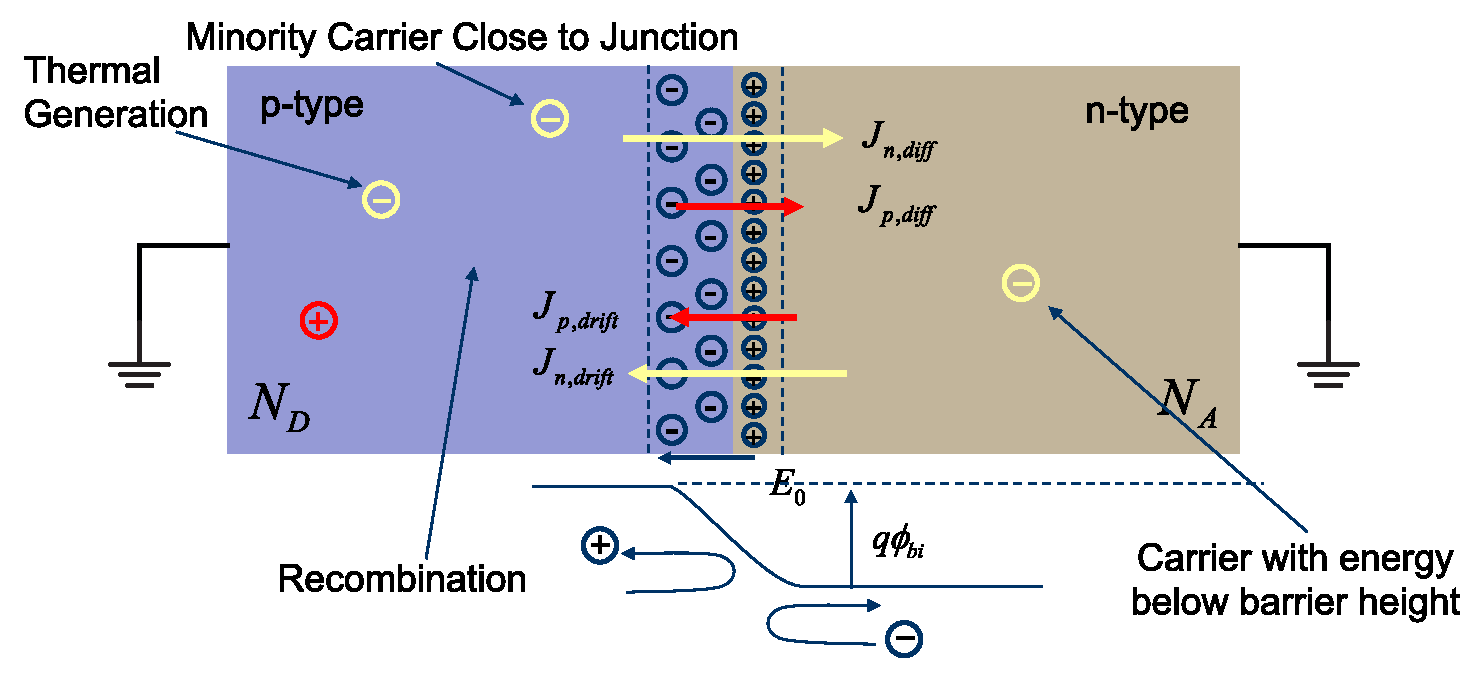
\includegraphics[width=.75\columnwidth]{slide35}
\caption{In equilibrium, with no applied fields, the current in a $PN$-junction is zero because drift and diffusion current cancel.  The built-in potential only allows a small diffusion current to flow, and drift currents due to minority carriers flow in the opposite direction.}
\label{fig:slide35}
\end{figure}
%%%%%%%%%%%%%%%%%%%%%%%%%%%%%%%%%%%%%%%%%%%%
Under thermal equilibrium (Fig.~\ref{fig:slide35}), when there's no bias, we know that the net current is zero.  The diffusion current is small since few carriers have enough energy to penetrate the barrier.   Drift current is small since minority carriers are few and far between, and only minority carriers generated within a diffusion length can contribute current.  Other minority carriers recombine before they reach the junction.
%%%%%%%%%%%%%%%%%%%%%%%%%%%%%%%%%%%%%%%%%%%%
%             SUBSECTION 6.2.2             %
%%%%%%%%%%%%%%%%%%%%%%%%%%%%%%%%%%%%%%%%%%%%
\subsection{Reverse Bias}
There are two important points to keep in mind.  First, minority drift current is independent of the barrier height, or the built-in potential between the p-n junction.  On the other hand, diffusion current is a strong (exponential) function of the barrier height.  Since a reverse bias causes an increased barrier to diffusion, as shown in Fig.~\ref{fig:slide36}, the diffusion current is reduced exponentially.  The drift current does not change, so the net result is a small reverse current, known as the ``saturation current".  
%%%%%%%%%%%%%%%%%%%%%%%%%%%%%%%%%%%%%%%%%%%%
%                 FIGURE                   %
%%%%%%%%%%%%%%%%%%%%%%%%%%%%%%%%%%%%%%%%%%%%
\begin{figure}[tb]
\centering
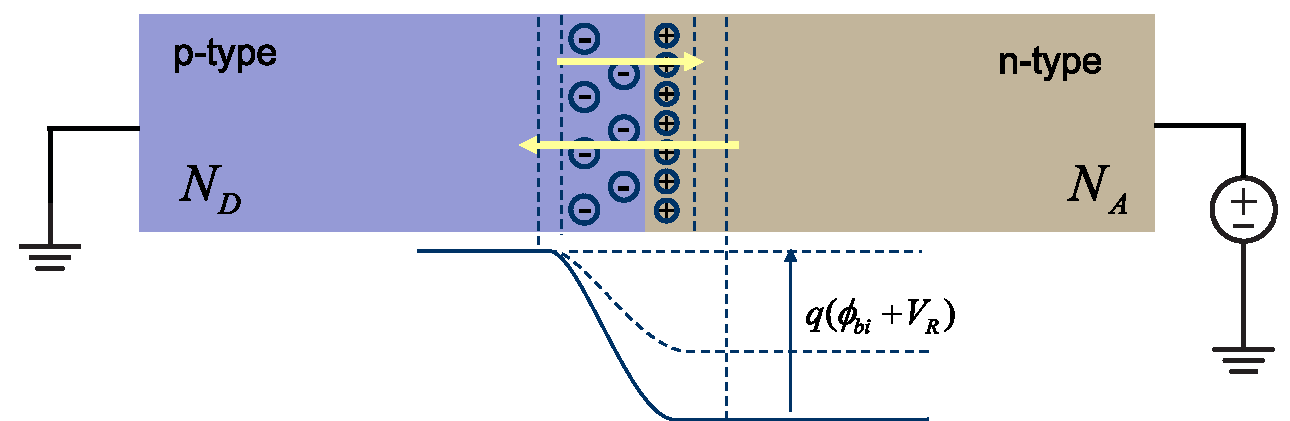
\includegraphics[width=.75\columnwidth]{slide36}
\caption{When a reverse bias is applied across a $PN$-junction, the diffusion current reduces (exponentially), and so drift currents overcome diffusion currents.  The drift currents are usually very small since they are a result of minority carriers that are generated near the junction.}
\label{fig:slide36}
\end{figure}
%%%%%%%%%%%%%%%%%%%%%%%%%%%%%%%%%%%%%%%%%%%%
%             SUBSECTION 6.2.3             %
%%%%%%%%%%%%%%%%%%%%%%%%%%%%%%%%%%%%%%%%%%%%
\subsection{Forward Bias}
With reference to Fig.~\ref{fig:slide36b}, a forward bias causes an exponential increase in the number of carriers with sufficient energy to penetrate barrier, and so the diffusion current \textbf{\textit{increases}} exponentially.  As the drift current does not change, the net result is a large forward current.
%%%%%%%%%%%%%%%%%%%%%%%%%%%%%%%%%%%%%%%%%%%%
%                 FIGURE                   %
%%%%%%%%%%%%%%%%%%%%%%%%%%%%%%%%%%%%%%%%%%%%
\begin{figure}[tb]
\centering
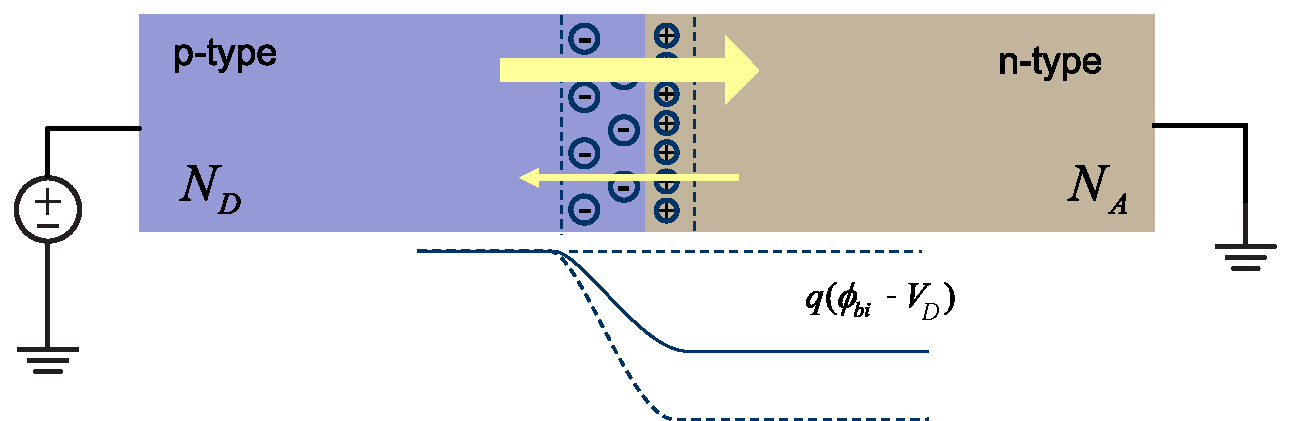
\includegraphics[width=.75\columnwidth]{slide36b}
\caption{In forward bias, the diffusion current increases (exponentially) and dominates over the drift current from minority carriers.  Majority carriers from the $P$-region are injected into the $N$-type region and become minority carriers. The same happens to electrons injected from the $N$-side.}
\label{fig:slide36b}
\end{figure}
%%%%%%%%%%%%%%%%%%%%%%%%%%%%%%%%%%%%%%%%%%%%
%             SUBSECTION 6.2.4             %
%%%%%%%%%%%%%%%%%%%%%%%%%%%%%%%%%%%%%%%%%%%%
\subsection{Diode I-V Curve}
%%%%%%%%%%%%%%%%%%%%%%%%%%%%%%%%%%%%%%%%%%%%
%                 FIGURE                   %
%%%%%%%%%%%%%%%%%%%%%%%%%%%%%%%%%%%%%%%%%%%%
\begin{figure}[tb]
\centering
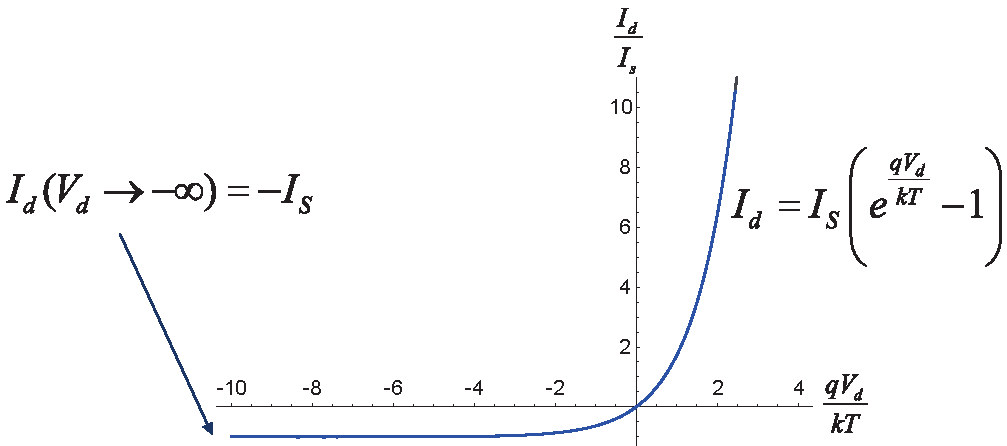
\includegraphics[width=.75\columnwidth]{slide38}
\caption{The $I$-$V$ curve for a diode.  The diode voltage is normalized to $kT/q$ and the current is normalized to the diode saturation current $I_S$.   In forward bias, the current increases exponentially whereas in reverse bias the current saturates to a small value of $I_S$.}
\label{fig:slide38}
\end{figure}
%%%%%%%%%%%%%%%%%%%%%%%%%%%%%%%%%%%%%%%%%%%%
As shown in Fig.~\ref{fig:slide38}, the diode $I-V$ relation is an exponential function, as we have discussed qualitatively.    This exponential is due to the Boltzmann distribution of carrier number versus energy.    For a reverse bias voltage,  the current saturates to $I_S$, the bias independent drift current due to minority carriers.
%%%%%%%%%%%%%%%%%%%%%%%%%%%%%%%%%%%%%%%%%%%%
%             SUBSECTION 6.2.5             %
%%%%%%%%%%%%%%%%%%%%%%%%%%%%%%%%%%%%%%%%%%%%
\subsection{Fabrication of IC Diodes}
%%%%%%%%%%%%%%%%%%%%%%%%%%%%%%%%%%%%%%%%%%%%
%                 FIGURE                   %
%%%%%%%%%%%%%%%%%%%%%%%%%%%%%%%%%%%%%%%%%%%%
\begin{figure}[tb]
\centering
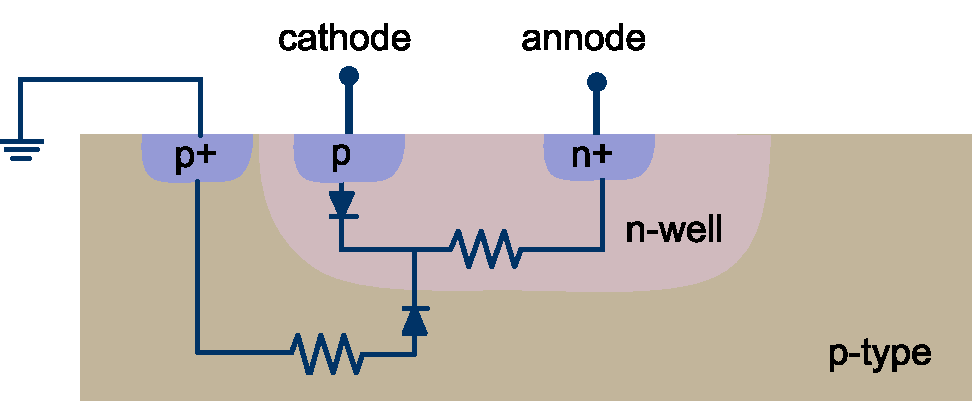
\includegraphics[width=.65\columnwidth]{slide44}
\caption{Cross section of a fabricated IC diode.  The n-well is used to isolate the diode from the substrate and the diffusion regions inside the n-well are used for the diode structure.  The cathode is connected to a p region that forms the pn junction with the n-well, and the n$^+$ region is used to make an ohmic contact with the n-well.  The substrate is biased to the most negative voltage to prevent the parasitic diode (n-well to substrate) from forward biasing.}
\label{fig:slide44}
\end{figure}
%%%%%%%%%%%%%%%%%%%%%%%%%%%%%%%%%%%%%%%%%%%%
Our drawings of $PN$-junctions so far has been very idealized.  The actual structure of a $PN$-junction is slightly more complex, as shown in Fig.~\ref{fig:slide44}.  To fabricate a diode, we first start with $P$-type substrate (typically).  We create an ``n-well" diffusion region  to house the diode.  Within the well, we counter dope to create p and n$^+$ diffusion regions to form  the cathode and anode terminals of the diode.  The n$^+$ region may seem puzzling at first, but it's needed to create an ohmic contact with the metal region at the anode.  Note that we actually end up with two diodes, one between the cathode and anode, as desired, and one from the substrate to the n-well region, which is a parasitic diode.  Why not use this diode?  The reason is that in an integrated circuit, we have many components and we want them to be isolated from each other.  Since all circuits fabricated share the silicon substrate, the substrate node is usually not used.  But a diode is a diode, and to isolate the devices from one another, we must reverse bias the unwanted diodes.  In this case, the n-well must be reverse biased with respect to the substrate.  Typically the substrate is tied to the lowest potential (ground for example) using substrate ``taps" or body contacts, which are p$^+$ regions as shown.  One final word about a practical diode.  We have drawn in resistors to remind ourselves that $P$-type and $N$-type regions are resistive and if we are not careful, resistive parasitics will add up and dominate the device behavior.  
%%%%%%%%%%%%%%%%%%%%%%%%%%%%%%%%%%%%%%%%%%%%%%%%%%%%%%%%%%%%%%%%%%%%%%%%%%%%%%%%%%%%%%%%
%%%%%%%%%%%%%%%%%%%%%%%%%%%%%%%%%%%%%%%%%%%%%%%%%%%%%%%%%%%%%%%%%%%%%%%%%%%%%%%%%%%%%%%%
%                                   SECTION 6.3                                        %
%%%%%%%%%%%%%%%%%%%%%%%%%%%%%%%%%%%%%%%%%%%%%%%%%%%%%%%%%%%%%%%%%%%%%%%%%%%%%%%%%%%%%%%%
%%%%%%%%%%%%%%%%%%%%%%%%%%%%%%%%%%%%%%%%%%%%%%%%%%%%%%%%%%%%%%%%%%%%%%%%%%%%%%%%%%%%%%%%
\section{Carrier concentration in Non-Equilibrium}
%%%%%%%%%%%%%%%%%%%%%%%%%%%%%%%%%%%%%%%%%%%%
%             SUBSECTION 6.3.1             %
%%%%%%%%%%%%%%%%%%%%%%%%%%%%%%%%%%%%%%%%%%%%
\subsection{Equilibrium versus Non-Equilibrium}
The Law of Mass Action says that in equilibrium, the product of the concentration of holes and electrons is constant
    \begin{equation}
        n \times p = n_i^2
    \end{equation}
As you may recall, we derived (in a hand wavy fashion) this equation by asserting that in equilibrium, the rate of generation and recombination should be equal.  We identified the left-hand side as proportional to the recombination rate (the more carriers, the more recombination):
    \begin{equation}
        R = c\,\, n \cdot p 
    \end{equation}
and the right hand side as the thermal generation rate:
    \begin{equation}
        G = \text{constant} = f(T) 
    \end{equation}
By equating these two, we have the Law of Mass Action:
    \begin{equation}
        R = G \Rightarrow n \cdot p = n_i^2(T) 
    \end{equation}
Since the thermal generation rate is essentially a constant for a fixed temperature, if an external process drives up the concentration of say one type of carriers, in particular minority carriers, then we can say that we are in a non-equilibrium situation because now there is an imbalance between recombination and generation:  
    \begin{equation}
        R \ne G 
    \end{equation}
The rate of thermal generation is the same as before, but now we have an excess of minority carriers: 
    \begin{equation}
        R > G 
    \end{equation}
What happens? The extra carriers should recombine at a higher rate and in steady-state we should return to equilibrium.  What drives the dynamics ?
%%%%%%%%%%%%%%%%%%%%%%%%%%%%%%%%%%%%%%%%%%%%
%             SUBSECTION 6.3.2             %
%%%%%%%%%%%%%%%%%%%%%%%%%%%%%%%%%%%%%%%%%%%%
\subsection{Recombination-Generation Centers}
%%%%%%%%%%%%%%%%%%%%%%%%%%%%%%%%%%%%%%%%%%%%
%                 FIGURE                   %
%%%%%%%%%%%%%%%%%%%%%%%%%%%%%%%%%%%%%%%%%%%%
\begin{figure}[tb]
\centering
\begin{tabular}{cc}
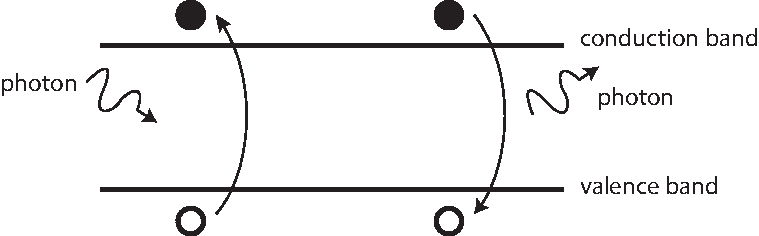
\includegraphics[width=.45\columnwidth]{gr_direct} &
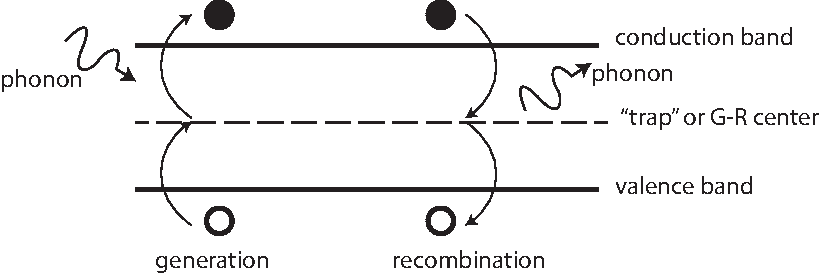
\includegraphics[width=.45\columnwidth]{gr_indirect}\\
(a) & (b)\\
\end{tabular}
\caption{(a) Direct generation and recombination by aid of an optical photon with energy exceeding the band gap.  (b)  Trap assisted generation and recombination through vacancies, defects, or impurities with approximately mid-band gap energy levels.  In silicon, the process in (b) is much more common. } \label{fig:gr_direct}
\end{figure}
%%%%%%%%%%%%%%%%%%%%%%%%%%%%%%%%%%%%%%%%%%%%
Up to now we have assumed that all generation and recombination occurs through a direct mechanism (shown on the left of Fig.~\ref{fig:gr_direct}) whereby valence band electrons accept energy (thermal or optical) and are raised into the conduction band.  The inverse process is of course recombination. This direct mechanism, while possible, is very unlikely in silicon. In reality most recombination and generation occurs through an indirect mechanism shown on the right of the figure.  The energy level near the middle of the band represents a ``trap", usually an impurity or missing atom in the crystal, that can assist both processes by temporarily trapping an electron and then releasing it into the valence band (and vice versa). This process captures and releases phonons (crystal vibrations) rather than optical photons.
%%%%%%%%%%%%%%%%%%%%%%%%%%%%%%%%%%%%%%%%%%%%
%             SUBSECTION 6.3.3             %
%%%%%%%%%%%%%%%%%%%%%%%%%%%%%%%%%%%%%%%%%%%%
\subsection{Thermal Generation/Recombination Rate}
For a hole in an $N$-type material, we find the rate of generation is given by
    \begin{equation}
        \left. \frac{\partial \Delta p}{\partial t} \right|_{\text{thermal R-G}} = - c_p N_T \Delta p
    \end{equation}
In the above equation, we have partial derivatives because there are many mechanisms that generate carriers, we are just focusing on the thermal rate.  $\Delta p$ is the excess minority carrier concentration above equilibrium
    \begin{equation}
        \Delta p = p - p_0
    \end{equation}
Here the rate is negative when $\Delta p > 0$ because recombination will outweigh generation when we create an excess of minority carriers.  Note that the rate depends on a constant $c_p$, the density of traps $N_T$, and the number of excess minority carriers $\Delta p$.  
%%%%%%%%%%%%%%%%%%%%%%%%%%%%%%%%%%%%%%%%%%%%
%              SUB-SUBSECTION              %
%%%%%%%%%%%%%%%%%%%%%%%%%%%%%%%%%%%%%%%%%%%%
\subsubsection*{Minority Carrier Lifetime}
It's common practice to lump the constants $c_p N_T$ into a term called the minority carrier lifetime $\tau_p$, because from the above equation it's clear that their product has units of inverse time.
    \begin{equation}
        \left. \frac{\partial \Delta p}{\partial t} \right|_{\text{thermal R-G}} = - c_p N_T \Delta p = - \frac{\Delta p}{\tau_p}
        \label{eq:lifetime}
    \end{equation} 
The minority carrier lifetime depends very strongly on the quality of the material and can vary by orders of magnitude for a poorly controlled process to a well controlled one (from nanoseconds to microseconds).
%%%%%%%%%%%%%%%%%%%%%%%%%%%%%%%%%%%%%%%%%%%%
%              SUB-SUBSECTION              %
%%%%%%%%%%%%%%%%%%%%%%%%%%%%%%%%%%%%%%%%%%%%
\subsubsection*{Majority Carriers versus Minority Carriers}
Equation~\ref{eq:lifetime} can be interpreted as the ``lifetime" of a minority carrier.  We know minority carriers ``live" in a pool of majority carriers and they annihilate upon meeting majority carriers.  When you're a minority carrier, there's a good chance that you're going to recombine with a majority carrier, especially when there are more traps $N_T$.  The more minority carriers there are, the faster the rate of recombination.  Note the rate of generation is fixed (towards equilibrium) whereas the recombination rate is higher due to the excess carriers.  The same equation is of course valid for electrons in a $P$-type region
    \begin{equation}
        \left. \frac{\partial \Delta n}{\partial t} \right|_{\text{thermal R-G}} = - \frac{\Delta n}{\tau_n}
    \end{equation}
%%%%%%%%%%%%%%%%%%%%%%%%%%%%%%%%%%%%%%%%%%%%%%%%%%%%%%%%%%%%%%%%%%%%%%%%%%%%%%%%%%%%%%%%
%%%%%%%%%%%%%%%%%%%%%%%%%%%%%%%%%%%%%%%%%%%%%%%%%%%%%%%%%%%%%%%%%%%%%%%%%%%%%%%%%%%%%%%%
%                                   SECTION 6.4                                        %
%%%%%%%%%%%%%%%%%%%%%%%%%%%%%%%%%%%%%%%%%%%%%%%%%%%%%%%%%%%%%%%%%%%%%%%%%%%%%%%%%%%%%%%%
%%%%%%%%%%%%%%%%%%%%%%%%%%%%%%%%%%%%%%%%%%%%%%%%%%%%%%%%%%%%%%%%%%%%%%%%%%%%%%%%%%%%%%%%
\section{Current Continuity Equation}
%%%%%%%%%%%%%%%%%%%%%%%%%%%%%%%%%%%%%%%%%%%%
%             SUBSECTION 6.4.1             %
%%%%%%%%%%%%%%%%%%%%%%%%%%%%%%%%%%%%%%%%%%%%
\subsection{Excess Carrier Continuity}
%%%%%%%%%%%%%%%%%%%%%%%%%%%%%%%%%%%%%%%%%%%%
%                 FIGURE                   %
%%%%%%%%%%%%%%%%%%%%%%%%%%%%%%%%%%%%%%%%%%%%
\begin{figure}[tb]
\centering
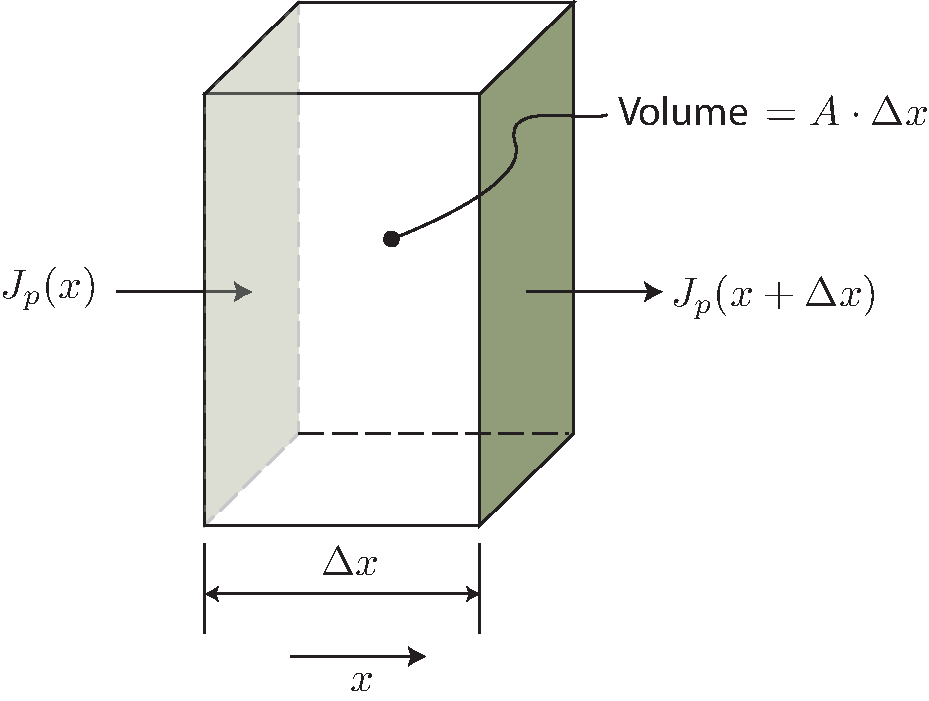
\includegraphics[width=.65\columnwidth]{Jbox}
\caption{Current flow into a region must satisfy the continuity equation.  If the current density varies spatially, it must be accompanied by generation or recombination.}
\label{fig:Jbox}
\end{figure}
%%%%%%%%%%%%%%%%%%%%%%%%%%%%%%%%%%%%%%%%%%%%
Consider a ``box" of current flowing shown in Fig.~\ref{fig:Jbox}.  Note that if the current density varies spatially (assume variations along $yz$ are negligible), then there must be a net rate of accumulation (or depletion) of carriers.  Applying this to excess minority carriers, we have
    \begin{equation}
        J_p(x + \Delta x) - J_p(x) =  \Delta x q \frac{\partial \Delta p}{\partial t} =  \Delta x q \frac{\Delta p}{\tau_p}
    \end{equation}
This equation is stating something quite obvious.  If the number of minority carriers is changing within a region, then there must be either generation or recombination in that region.  We known from our previous discussion that the excess minority carrier population varies as $\Delta p/\tau_p$.
%%%%%%%%%%%%%%%%%%%%%%%%%%%%%%%%%%%%%%%%%%%%
Now taking $\Delta x \rightarrow 0$, we have the following differential equation
    \begin{equation}
        \frac{dJ_p}{dx}  = q \frac{\Delta p}{\tau_p}
    \end{equation}
%%%%%%%%%%%%%%%%%%%%%%%%%%%%%%%%%%%%%%%%%%%%
%             SUBSECTION 6.4.2             %
%%%%%%%%%%%%%%%%%%%%%%%%%%%%%%%%%%%%%%%%%%%%
\subsection{Diffusion Currents}
Now we also know that if there's a spatial variation in the concentration of carriers, then we also have to account for a diffusion current
    \begin{equation}
        J_p = q D_p \frac{d\Delta p}{dx}
    \end{equation}
Putting this all together, we have 
    \begin{equation}
        \frac{dJ_p}{dx}  = \frac{d(q D_p \frac{d\Delta p}{dx})}{dx} = q D_p \frac{d^2 \Delta  p}{dx^2} = q \frac{\Delta p}{\tau_p}
    \end{equation}
Simplifying the equation, and defining a new constant $L_p$, we have
    \begin{equation}
        \frac{d^2 \Delta p}{dx^2} =  \frac{\Delta p}{D_p \tau_p} =  \frac{\Delta p}{L_p^2}
        \label{eq:continuity}
    \end{equation}
The constant $L_p = \sqrt{D_p \tau_p}$ is known as the diffusion length for reasons which will become clear shortly.
%%%%%%%%%%%%%%%%%%%%%%%%%%%%%%%%%%%%%%%%%%%%
%             SUBSECTION 6.4.3             %
%%%%%%%%%%%%%%%%%%%%%%%%%%%%%%%%%%%%%%%%%%%%
\subsection{Excess Carrier Current Flow}
%%%%%%%%%%%%%%%%%%%%%%%%%%%%%%%%%%%%%%%%%%%%
%                 FIGURE                   %
%%%%%%%%%%%%%%%%%%%%%%%%%%%%%%%%%%%%%%%%%%%%
\begin{figure}[tb]
\centering
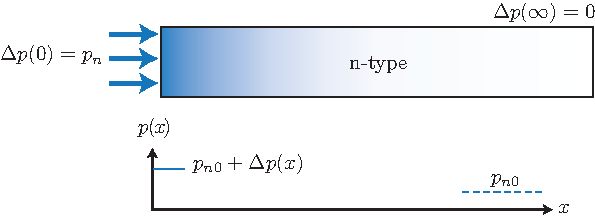
\includegraphics[width=.75\columnwidth]{excess_charge_inject}
\caption{Excess minority carrier charge is continuously injected at the origin into an $N$-type region.  Far away from the injection, we expect carriers to return to equilibrium values.  Using these boundary points, we would like to solve for the minority carrier distribution in the $N$-type region.} \label{fig:excess_charge_inject}
\end{figure}
%%%%%%%%%%%%%%%%%%%%%%%%%%%%%%%%%%%%%%%%%%%%
Let's suppose that some process, yet to be determined, continually creates an excess of minority carriers at the origin of an $N$-type semiconductor (shown in Fig.~\ref{fig:excess_charge_inject}).  In other words, the boundary conditions are
    \begin{equation}
        \Delta p(0) = p_{n}
    \end{equation}	
and
    \begin{equation}
        \Delta p(\infty) = 0
    \end{equation}	
where we assume that the ``disturbance" at $x$ is maintained over all time (steady-state) and that far away from the disturbance, thermal equilibrium conditions persist.  What's the distribution of carriers as we leave the origin?  
%%%%%%%%%%%%%%%%%%%%%%%%%%%%%%%%%%%%%%%%%%%%
%              SUB-SUBSECTION              %
%%%%%%%%%%%%%%%%%%%%%%%%%%%%%%%%%%%%%%%%%%%%
\subsubsection*{Minority Carrier Distribution}
%%%%%%%%%%%%%%%%%%%%%%%%%%%%%%%%%%%%%%%%%%%%
%                 FIGURE                   %
%%%%%%%%%%%%%%%%%%%%%%%%%%%%%%%%%%%%%%%%%%%%
\begin{figure}[tb]
\centering
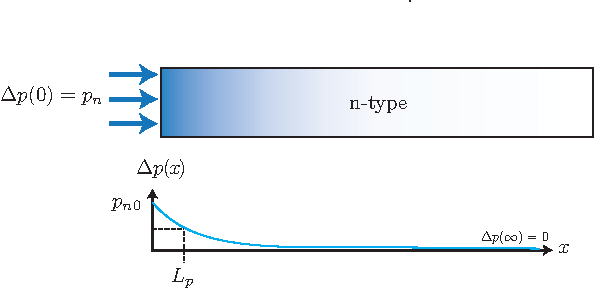
\includegraphics[width=.75\columnwidth]{excess_charge_inject_sol}
\caption{Minority carrier distribution as a function of position when excess carriers are continuously injected at the origin.}
\label{fig:excess_charge_inject_sol}
\end{figure}
%%%%%%%%%%%%%%%%%%%%%%%%%%%%%%%%%%%%%%%%%%%%
The general solution, shown in Fig.~\ref{fig:excess_charge_inject_sol}, is given by
    \begin{equation}
        \Delta p(x) = A e^{-x/L_p} + B e^{x/L_p}
    \end{equation}	
 Applying boundary conditions, we have $B = 0$ and $A = p_{n}$
    \begin{equation}
        \Delta p(x) = p_n e^{-x/L_p} 
    \end{equation}	
which also satisfies the $\Delta p(\infty)$ boundary condition.  It's important to realize this is a steady-state solution (there's no time dependence).   
%%%%%%%%%%%%%%%%%%%%%%%%%%%%%%%%%%%%%%%%%%%%
%              SUB-SUBSECTION              %
%%%%%%%%%%%%%%%%%%%%%%%%%%%%%%%%%%%%%%%%%%%%
\subsubsection*{Majority and Minority Carrier Distribution}
We can find the current flow due to this excess minority concentration by calculating the diffusion current
    \begin{equation}
        J_p(x) = -q D_p \frac{d \Delta p}{dx} = \frac{p_n}{L_p} e^{-x/L_p} 
    \end{equation}	
Which shows that the excess minority carriers diffuse into the $N$-type region a distance of a few $L_p$.  Note that the current density varies with $x$.  Yet the current must be continuous because charge is not piling up as a function of time.  Recall this is a steady-state distribution.  This means that if we evaluate the current at $x = 0$, that's the same current found throughout the $N$-type region. 
%%%%%%%%%%%%%%%%%%%%%%%%%%%%%%%%%%%%%%%%%%%%
Where is the additional current coming from?  It's coming from majority carriers who are ``coming in" to annihilate the minority carriers.  They contribute a current which is exactly $1- J_p(x)$.  
%%%%%%%%%%%%%%%%%%%%%%%%%%%%%%%%%%%%%%%%%%%%%%%%%%%%%%%%%%%%%%%%%%%%%%%%%%%%%%%%%%%%%%%%
%%%%%%%%%%%%%%%%%%%%%%%%%%%%%%%%%%%%%%%%%%%%%%%%%%%%%%%%%%%%%%%%%%%%%%%%%%%%%%%%%%%%%%%%
%                                   SECTION 6.5                                        %
%%%%%%%%%%%%%%%%%%%%%%%%%%%%%%%%%%%%%%%%%%%%%%%%%%%%%%%%%%%%%%%%%%%%%%%%%%%%%%%%%%%%%%%%
%%%%%%%%%%%%%%%%%%%%%%%%%%%%%%%%%%%%%%%%%%%%%%%%%%%%%%%%%%%%%%%%%%%%%%%%%%%%%%%%%%%%%%%%
\section{Forward Biased $PN$-junctions}
%%%%%%%%%%%%%%%%%%%%%%%%%%%%%%%%%%%%%%%%%%%%
%             SUBSECTION 6.5.1             %
%%%%%%%%%%%%%%%%%%%%%%%%%%%%%%%%%%%%%%%%%%%%
\subsection{Minority Carriers at Junction Edges}
When a diode is at zero bias, we know that the diffusion and drift currents balance.  If we forward bias the junction, then we are lowering the barrier to diffusion current flow, which means more minority carriers will be injected.  The exact derivation leads to the following expression for the minority carrier concentration at boundaries of the depletion region :
    \begin{equation} 
        \frac{{{p_n}(x = {x_n})}}{{{p_p}(x =  - {x_p})}} =  {e^{ - (Barrier\,Energy)/kT}}
    \end{equation}
The result is known as Boltzmann's Law:
    \framebox{$
    \frac{{{p_n}(x = {x_n})}}{{{N_A}}} = {e^{ - q({\varphi _{bi}} - {V_D})/kT}}$}, where $V_D$ is the forward bias voltage that we apply, and $\varphi_{bi}$ is the built-in potential.  This implies an exponentially larger number of minority carriers that are injected into the regions.
%%%%%%%%%%%%%%%%%%%%%%%%%%%%%%%%%%%%%%%%%%%%
We actually derived this equation in the last chapter under thermal equilibrium, but it's important to realize that we're now in a non-equilibrium situation.  So strictly speaking, our derivation does not apply.  In practice, it can be shown that under ``low level injection" conditions, in other words, when the density of minority carriers injected remains much smaller than the number of majority carriers, the law is valid.
%%%%%%%%%%%%%%%%%%%%%%%%%%%%%%%%%%%%%%%%%%%%
Using Boltzmann's Law, the minority carrier concentrations at the edges of the depletion region are given by:
    \begin{equation} 
        {p_n}(x = {x_n}) = {N_A}{e^{ - q({\varphi _B} - {V_D})/kT}}
    \end{equation}
    \begin{equation} 
        {n_p}(x =  - {x_p}) = {N_D}{e^{ - q({\varphi _B} - {V_D})/kT}}
    \end{equation}
Here are some important things to remember about these equations.  In particular, the subscript notation is confusing at first, so please study each term in the above equation carefully.
    \begin{itemize}
        \item Note 1: $N_A$ and $N_D$ are the majority carrier concentrations on the \textit{other} side of the junction.
        \item  Note 2: We can reduce these equations further by substituting $V_D = 0$V and verifying that we satisfy thermal equilibrium conditions.
        \item  Note 3:  These equations are valid assuming that $p_n \ll N_D$ and $n_p \ll N_A$
    \end{itemize}
%%%%%%%%%%%%%%%%%%%%%%%%%%%%%%%%%%%%%%%%%%%%
%             SUBSECTION 6.5.2             %
%%%%%%%%%%%%%%%%%%%%%%%%%%%%%%%%%%%%%%%%%%%%
\subsection{Minority Carrier Concentration Distribution}
%%%%%%%%%%%%%%%%%%%%%%%%%%%%%%%%%%%%%%%%%%%%
%                 FIGURE                   %
%%%%%%%%%%%%%%%%%%%%%%%%%%%%%%%%%%%%%%%%%%%%
\begin{figure}[tb]
\centering
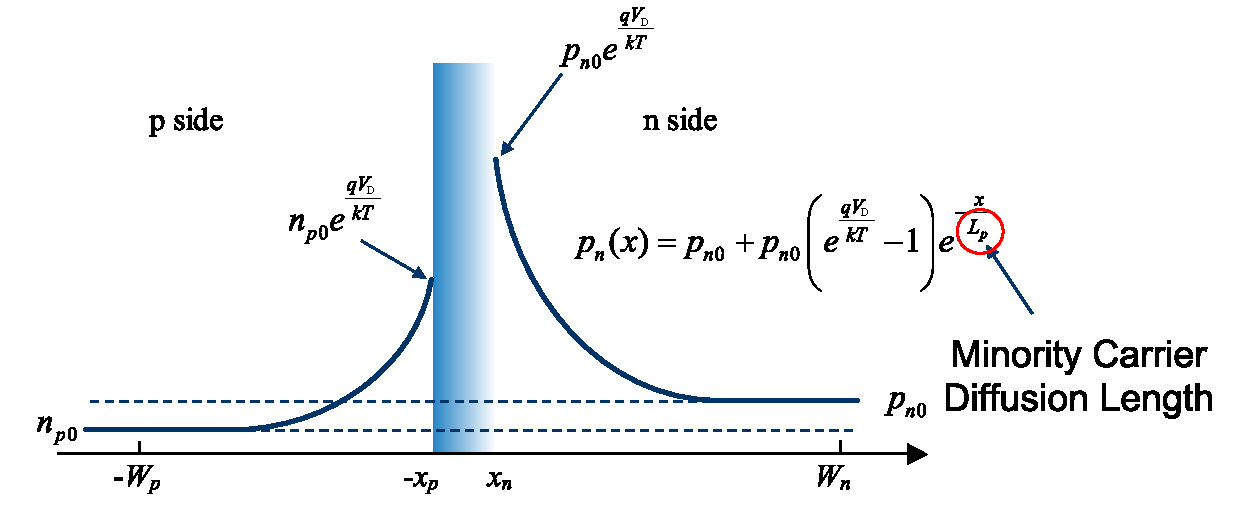
\includegraphics[width=.75\columnwidth]{slide41}
\caption{Distribution of minority carriers in a $PN$-junction under forward bias.  Forward bias increases the diffusion current and causes excess minority carriers (above thermal equilibrium values) to be injected into the p and n type regions.  The minority carriers diffuse and recombine and exhibit an exponentially decaying profile.}
\label{fig:slide41}
\end{figure}
%%%%%%%%%%%%%%%%%%%%%%%%%%%%%%%%%%%%%%%%%%%%
With an excess of minority currents injected into the n and p regions, we can use our previously derived result to find the carrier concentration as a function of $x$.  Note that the currents decay exponentially with a characteristic length corresponding to the diffusion length.  The solutions are plotted in Fig.~\ref{fig:slide41}.
%%%%%%%%%%%%%%%%%%%%%%%%%%%%%%%%%%%%%%%%%%%%
%                 FIGURE                   %
%%%%%%%%%%%%%%%%%%%%%%%%%%%%%%%%%%%%%%%%%%%%
\begin{figure}[tb]
\centering
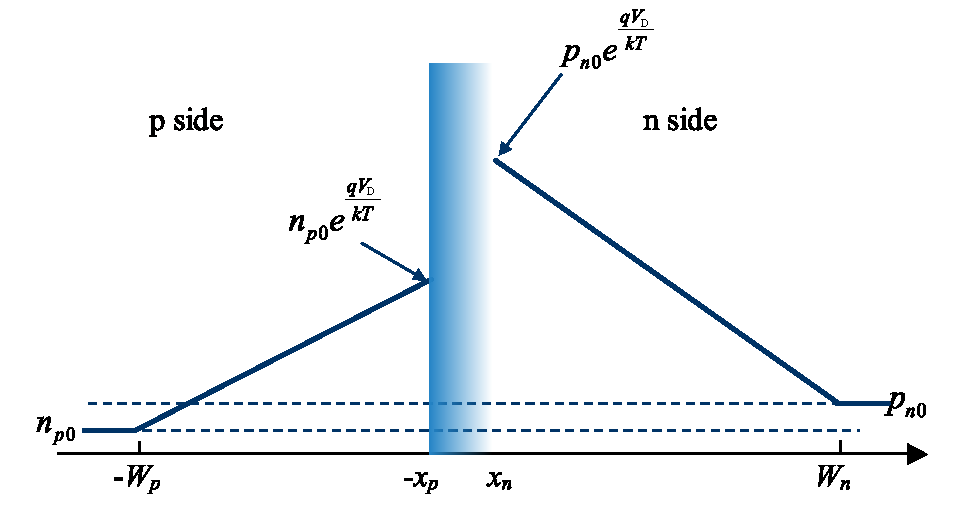
\includegraphics[width=.75\columnwidth]{slide42}
\caption{Distribution of minority carriers in a $PN$-junction under forward bias for the case of very long minority carrier lifetime.  The minority carriers diffuse but do not recombine with majority carriers, leading to linear gradients in the profile.}
\label{fig:slide42}
\end{figure}
%%%%%%%%%%%%%%%%%%%%%%%%%%%%%%%%%%%%%%%%%%%%
A special case, of great practical interest, is the case when virtually none of the diffusing holes and electrons recombine, in other words the material has a very long minority carrier lifetime.  The solution to the equations in this case can be rederived by taking the limit of large $\tau$.  The solution, shown in Fig.~\ref{fig:slide42}, is that we obtain straight lines for the concentration profile.
%%%%%%%%%%%%%%%%%%%%%%%%%%%%%%%%%%%%%%%%%%%%
To see this, solve the differential equation we derived earlier but set $\tau_p$ and $\tau_n$ to very large times.  This also happens if the minority carrier diffusion lengths are much larger than the diode width: $ {L_{n,p}} \gg {W_{n,p}} $.  Note that the form of the solution can be inferred if we note that without recombination, the current must be uniform, in other words the slope of the minority carrier profile \emph{must} be constant. That means that the carrier distribution is linear.
%%%%%%%%%%%%%%%%%%%%%%%%%%%%%%%%%%%%%%%%%%%%
%             SUBSECTION 6.5.3             %
%%%%%%%%%%%%%%%%%%%%%%%%%%%%%%%%%%%%%%%%%%%%
\subsection{Diode Diffusion Currents}
Given the profile of minority carrier currents in each region, it's rather straightforward to find the overall currents for holes and electrons.  Here we use the linear profile case to illustrate the calculations:
    \begin{equation}
        \frac{{d{n_p}}}{{dx}}(x) \approx \frac{{{n_{p0}}{e^{\frac{{q{V_A}}}{{kT}}}} - {n_{p0}}}}{{ - {x_p} - ( - {W_p})}}
    \end{equation}
Note that the electron minority carrier concentration at equilibrium is given by
    \begin{equation}
        {n_{p0}} = \frac{{n_i^2}}{{{N_A}}}
    \end{equation}
This leads to electron diffusion current
    \begin{equation}
        J_n^{diff} = q{D_n}{\left. {\frac{{d{n_p}}}{{dx}}} \right|_{x =  - {x_p}}} \approx q\frac{{{D_n}}}{{{W_p}}}{n_{p0}}\left( {{e^{\frac{{q{V_A}}}{{kT}}}} - 1} \right)
    \end{equation}
and hole diffusion current
    \begin{equation}
        J_p^{diff} =  - q{D_p}{\left. {\frac{{d{p_n}}}{{dx}}} \right|_{x = {x_n}}} \approx  - q\frac{{{D_p}}}{{{W_n}}}{p_{n0}}\left( {1 - {e^{\frac{{q{V_A}}}{{kT}}}}} \right)
    \end{equation}
Also, since electrons have negative charge, both electron and hole currents add in phase despite going in different directions to give a total current of
    \begin{equation}
        J_{}^{diff} = qn_i^2\left( {\frac{{{D_p}}}{{{N_D}{W_n}}} + \frac{{{D_n}}}{{{N_A}{W_p}}}} \right)\left( {{e^{\frac{{q{V_A}}}{{kT}}}} - 1} \right)
    \end{equation}
%%%%%%%%%%%%%%%%%%%%%%%%%%%%%%%%%%%%%%%%%%%%
%             SUBSECTION 6.5.4             %
%%%%%%%%%%%%%%%%%%%%%%%%%%%%%%%%%%%%%%%%%%%%
\subsection{Height Analogy}
%%%%%%%%%%%%%%%%%%%%%%%%%%%%%%%%%%%%%%%%%%%%
%                 FIGURE                   %
%%%%%%%%%%%%%%%%%%%%%%%%%%%%%%%%%%%%%%%%%%%%
\begin{figure}[tb]
\centering
\begin{tabular}{cc}
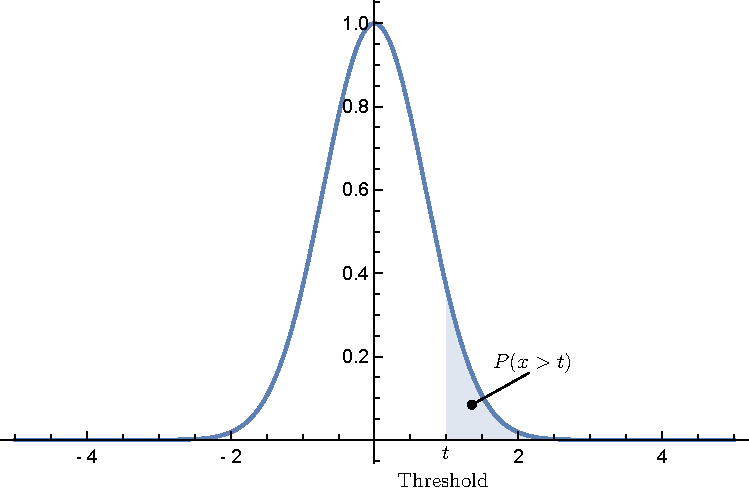
\includegraphics[width=.45\columnwidth]{norm4} &
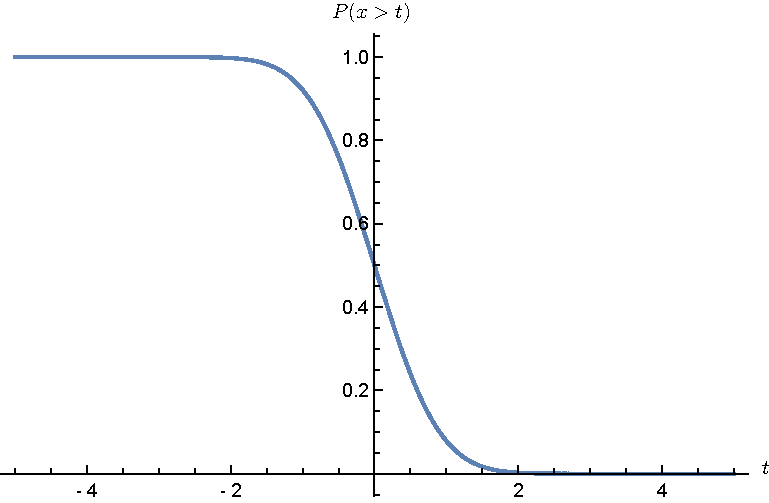
\includegraphics[width=.45\columnwidth]{erf}\\
(a) & (b)\\
\end{tabular}
\caption{(a) The normal distribution function (Gaussian distribution) is approximately the variation in heights between students on a playground.  The shaded area represents the fraction of students who are taller than a certain threshold.  (b)  The integration of the normal distribution as a function of threshold (the shaded area) shows that lowering the barrier (moving left along the curve) leads to an exponential increase in the number of students exceeding a threshold in height.}
\label{fig:norm4}
\end{figure}
%%%%%%%%%%%%%%%%%%%%%%%%%%%%%%%%%%%%%%%%%%%%
Imagine a ``wall" that is a certain height (say 6 feet tall) and imagine that if only kids in the playground are taller than a certain height can ``jump" the barrier.  This is the shaded area under the normal distribution, or the ``error function" plotted on the right (see Fig.~\ref{fig:norm4}).   From the plot, it's clear that as we decrease the height of the wall, exponentially more kids can jump the fence, because the shaded area is growing exponentially.  
%%%%%%%%%%%%%%%%%%%%%%%%%%%%%%%%%%%%%%%%%%%%%%%%%%%%%%%%%%%%%%%%%%%%%%%%%%%%%%%%%%%%%%%%
%%%%%%%%%%%%%%%%%%%%%%%%%%%%%%%%%%%%%%%%%%%%%%%%%%%%%%%%%%%%%%%%%%%%%%%%%%%%%%%%%%%%%%%%
%                                   SECTION 6.6                                        %
%%%%%%%%%%%%%%%%%%%%%%%%%%%%%%%%%%%%%%%%%%%%%%%%%%%%%%%%%%%%%%%%%%%%%%%%%%%%%%%%%%%%%%%%
%%%%%%%%%%%%%%%%%%%%%%%%%%%%%%%%%%%%%%%%%%%%%%%%%%%%%%%%%%%%%%%%%%%%%%%%%%%%%%%%%%%%%%%%
\section{Diode Small Signal Model}
In many applications, we are concerned with the diode response to a small signal.  In these situations, we usually bias the diode with a DC voltage to the desired operating point, either in forward or reverse biased region, and then we apply a small incremental signal to the diode.  A good example is when the diode is used as a switch, in which case we either turn the diode on and rely on its low impedance to pass small signals or turn it off to isolate small signals from the rest of the circuit. Many mobile phones use a diode exactly as described above to share a single antenna between the receiver and transmitter.  
%%%%%%%%%%%%%%%%%%%%%%%%%%%%%%%%%%%%%%%%%%%%
To understand how the forward biased diode responds to small signals, the $I-V$ relation of a diode is first approximated
    \begin{equation}
        {I_D} + {i_D} = {I_S}\left( {{e^{\frac{{q({V_d} + {v_d})}}{{kT}}}} - 1} \right) \approx {I_S}{e^{\frac{{q{V_d}}}{{kT}}}}{e^{\frac{{q{v_d}}}{{kT}}}}
    \end{equation}
For $x = v_d/kT/q$ and $v_d \ll kT/q$ (small-signals less than 26mV),  we can linearize the exponential using a Taylor Series expansion:
    \begin{equation}
        {e^x} = 1 + x + \frac{{{x^2}}}{{2!}} + \frac{{{x^3}}}{{3!}} +  \cdots 
    \end{equation}
In other words the total current can be written in terms of the DC bias current and the incremental AC current:
    \begin{equation}
        {I_D} + {i_D} \approx {I_D}\left( {1 + \frac{{q{v_d}}}{{kT}} +  \cdots } \right)
    \end{equation}
From the perspective of the ``small-signal", the current flows in proportion to the applied voltage $v_d$, in other words the diode looks like a conductor:
    \begin{equation}
        {i_D} \approx \frac{{q{v_d}}}{{kT}} = {g_d}{v_d}
    \end{equation}
%%%%%%%%%%%%%%%%%%%%%%%%%%%%%%%%%%%%%%%%%%%%
%             SUBSECTION 6.6.1             %
%%%%%%%%%%%%%%%%%%%%%%%%%%%%%%%%%%%%%%%%%%%%
\subsection{Diode Capacitance}
We have already seen that a reverse biased diode acts like a capacitor since the depletion region grows and shrinks in response to the applied field.  The capacitance in forward bias requires some additional derivations but in practice we can use the following approximation for the forward bias:
    \begin{equation}
        {C_j} = A\frac{{{\varepsilon _S}}}{{{X_{dep}}}} \approx 1.4C_{j0}
    \end{equation}
On the other hand, another important charge storage mechanism comes into play in forward bias.   Minority carriers injected into p and n regions “stay” in each region for a while.   On average additional charge is stored in diode that must be accounted form.
%%%%%%%%%%%%%%%%%%%%%%%%%%%%%%%%%%%%%%%%%%%%
%              SUB-SUBSECTION              %
%%%%%%%%%%%%%%%%%%%%%%%%%%%%%%%%%%%%%%%%%%%%
\subsubsection*{Charge Storage} \label{sec:charge_storage}
%%%%%%%%%%%%%%%%%%%%%%%%%%%%%%%%%%%%%%%%%%%%
%                 FIGURE                   %
%%%%%%%%%%%%%%%%%%%%%%%%%%%%%%%%%%%%%%%%%%%%
\begin{figure}[tb]
\centering
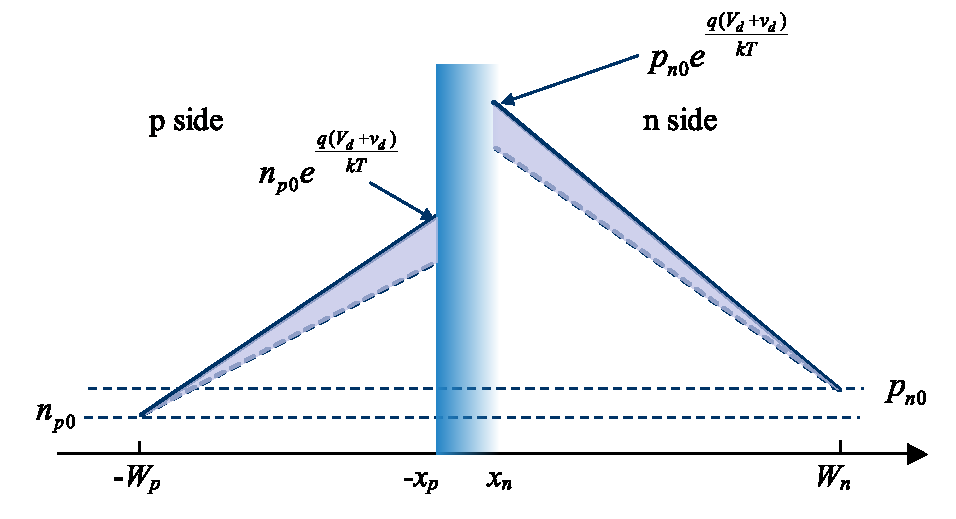
\includegraphics[width=.75\columnwidth]{slide47}
\caption{Change in minority carrier distribution in a forward biased diode when the forward bias is increased.  The dashed line represents the profile for a lower current, and the area between the curves represents the extra charge stored that must flow into the junction.}
\label{fig:slide47}
\end{figure}
%%%%%%%%%%%%%%%%%%%%%%%%%%%%%%%%%%%%%%%%%%%%
As shown in Fig.~\ref{fig:slide47}, increasing forward bias increases minority charge density (the area under the curve goes up).   By charge neutrality, the source voltage must supply equal and opposite charge. %%%%%%%%%%%%%%%%%%%%%%%%%%%%%%%%%%%%%%%%%%%%
A detailed analysis yields:
    \begin{equation}
        {C_d} = \frac{1}{2}\frac{{q{I_d}}}{{kT}}\tau
    \end{equation}
where  $\tau$ is either the time to cross junction (short junction) or the minority carrier lifetime (diffusion length shorter than width of diode).  
%%%%%%%%%%%%%%%%%%%%%%%%%%%%%%%%%%%%%%%%%%%%
Another way to understand why there's additional capacitance in the diode, imagine a voltage that abruptly transitions from forward bias to reverse bias.  If the diode were just a conductor, it would immediately shutoff, and the current would collapse to zero instantaneously.  Even accounting for the junction capacitance, the time to ``discharge" the diode must also account for the fact that the diffusion current is due to a spatial distribution of minority carriers in the p and n regions.  These distributions cannot collapse to equilibrium values instantaneously.  If we stop injecting carriers into the junction, then eventually the distribution will return to the equilibrium value, and the time is proportional to how long it takes for excess minority carriers to ``disappear", either through recombination or by leaving the diode.  This is why the capacitance is directly proportional to this time $\tau$, and also to the current.  The more current the diode is conducting, the more charge that is stored.  
%%%%%%%%%%%%%%%%%%%%%%%%%%%%%%%%%%%%%%%%%%%%
%             SUBSECTION 6.6.2             %
%%%%%%%%%%%%%%%%%%%%%%%%%%%%%%%%%%%%%%%%%%%%
\subsection{Complete Small-Signal Model}
%%%%%%%%%%%%%%%%%%%%%%%%%%%%%%%%%%%%%%%%%%%%
%                 FIGURE                   %
%%%%%%%%%%%%%%%%%%%%%%%%%%%%%%%%%%%%%%%%%%%%
\begin{figure}[tb]
\centering
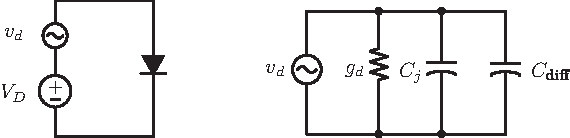
\includegraphics[width=.75\columnwidth]{diode_ss_model}
\caption{The complete small-signal model for a diode in forward bias includes diode conductance and charge storage capacitance due to the junction stored charge (depletion region width) and minority carrier stored charge.}
\label{fig:diode_ss_model}
\end{figure}
%%%%%%%%%%%%%%%%%%%%%%%%%%%%%%%%%%%%%%%%%%%%
In Fig.~\ref{fig:diode_ss_model}, we summarize everything about the diode small-signal model in the forward biased region in the form of an equivalent circuit.  We have seen that  from the perspective of the small-signal source, the diode appears as a resistor in parallel with a physical capacitor.    The above model is valid for a forward biased diode excited by a small \emph{incremental} signal.   It consists of three distinct components:  small-signal resistance, junction capacitance, and diffusion capacitance.  Strictly speaking, these components are non-linear as a function of operating point.  But for a fixed operating point, any small deviations around it ``see" linear components.
%%%%%%%%%%%%%%%%%%%%%%%%%%%%%%%%%%%%%%%%%%%%%%%%%%%%%%%%%%%%%%%%%%%%%%%%%%%%%%%%%%%%%%%%
%%%%%%%%%%%%%%%%%%%%%%%%%%%%%%%%%%%%%%%%%%%%%%%%%%%%%%%%%%%%%%%%%%%%%%%%%%%%%%%%%%%%%%%%
%                                   SECTION 6.7                                        %
%%%%%%%%%%%%%%%%%%%%%%%%%%%%%%%%%%%%%%%%%%%%%%%%%%%%%%%%%%%%%%%%%%%%%%%%%%%%%%%%%%%%%%%%
%%%%%%%%%%%%%%%%%%%%%%%%%%%%%%%%%%%%%%%%%%%%%%%%%%%%%%%%%%%%%%%%%%%%%%%%%%%%%%%%%%%%%%%%
\section{Photonic Applications}
%%%%%%%%%%%%%%%%%%%%%%%%%%%%%%%%%%%%%%%%%%%%
%             SUBSECTION 6.7.1             %
%%%%%%%%%%%%%%%%%%%%%%%%%%%%%%%%%%%%%%%%%%%%
\subsection{Solar Cells}
%%%%%%%%%%%%%%%%%%%%%%%%%%%%%%%%%%%%%%%%%%%%
%                 FIGURE                   %
%%%%%%%%%%%%%%%%%%%%%%%%%%%%%%%%%%%%%%%%%%%%
\begin{figure}[tb]
\centering
\includegraphics[width=.5\columnwidth]{solar_cell.jpg}
\caption{A typical solar panel is made from hundreds to thousands of diodes acting as photo-voltaic cells.}
\label{fig:solar_cell}
\end{figure}
%%%%%%%%%%%%%%%%%%%%%%%%%%%%%%%%%%%%%%%%%%%%
A solar cell is a $PN$-junction designed for converting light energy (photons) into electric energy (energized electrons).  It's also known as a photovoltaic cell (PV cell).  It's a common sight these days on rooftops and in solar farms (Fig.~\ref{fig:solar_cell}).   Typically efficiency numbers range from 10\% to 30\% and 1m$^2$ of area can generate at 25W of power on average (150W peak).  Also, the energy cost to fabricate a solar cell is steadily improving, and most solar panels will be energy neutral after a few years of operation.
%%%%%%%%%%%%%%%%%%%%%%%%%%%%%%%%%%%%%%%%%%%%
%             SUBSECTION 6.7.2             %
%%%%%%%%%%%%%%%%%%%%%%%%%%%%%%%%%%%%%%%%%%%%
\subsection{$PN$-junction Solar Cells}
%%%%%%%%%%%%%%%%%%%%%%%%%%%%%%%%%%%%%%%%%%%%
%                 FIGURE                   %
%%%%%%%%%%%%%%%%%%%%%%%%%%%%%%%%%%%%%%%%%%%%
\begin{figure}[tb]
\centering
\begin{tabular}{cc}
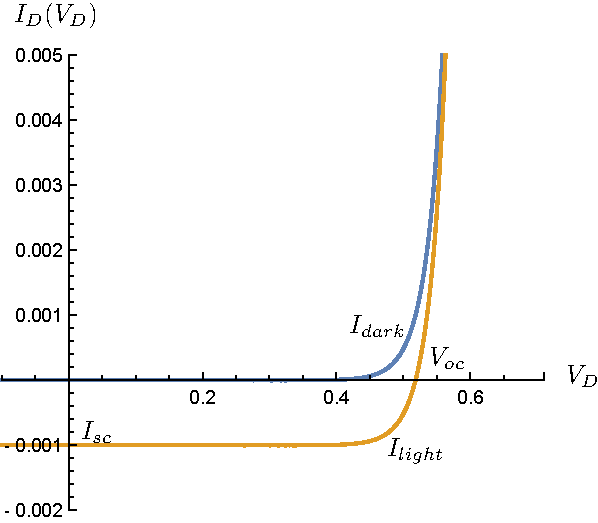
\includegraphics[width=.45\columnwidth]{solarcell_zoomout.pdf} &
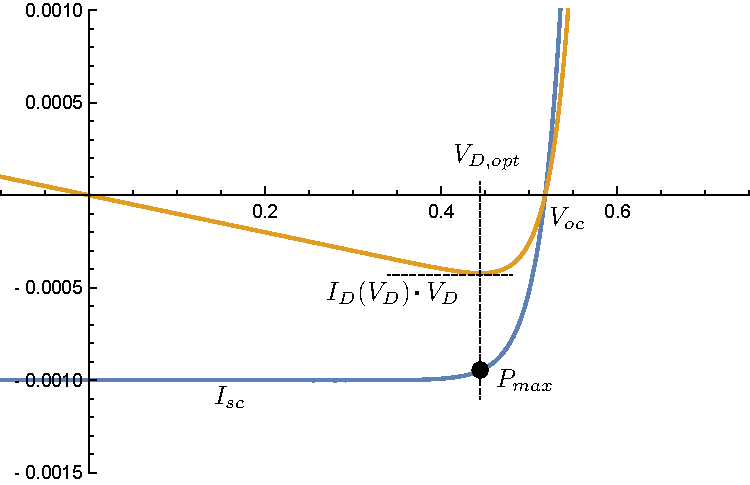
\includegraphics[width=.45\columnwidth]{solarcell.pdf}\\
(a) & (b)\\
\end{tabular}
\caption{(a) Modified diode $I$-$V$ curve to account for the photo-current.  (b)  A zoom in to the fourth quadrant where we can extract power from the photo-current.  The important parameters include the \emph{short circuit} current, the \emph{open circuit voltage}, and the point of maximum power $P_{max}$. }
\label{fig:solarcell_zoom}
\end{figure}
%%%%%%%%%%%%%%%%%%%%%%%%%%%%%%%%%%%%%%%%%%%%
The $I-V$ curve of a solar cell is basically the same as a diode with an extra ``generation" term  due to optical photons generating electron-hole pairs, as shown in Fig.~\ref{fig:solarcell_zoom}a.  The basic diode $I-V$ curve is modified to account for the photon generated carriers $I_{sc}$:
    \begin{equation} 
        I_D = I_S (e^{qV/kT} - 1) - I_{sc}
    \end{equation}
Up to now, we have been ignoring this photocurrent and so it's worthwhile to examine how to make this term significant.  Useful energy is only extracted when the $I\cdot V$ product is negative (here in the fourth quadrant), because in this region the solar cell is generating a voltage and current in opposite phase, and it's thereby a generator.\footnote{This is due to the passive sign convention that we adopt in electrical engineering and physics.}  If we zoom into the fourth quadrant (Fig.~\ref{fig:solarcell_zoom}b) and examine the product of $I\cdot V$, we can identify three important points.  The $I_{sc}$ is the current that flows when the voltage $V = 0$V, or for a short circuited solar cell.  Likewise, the voltage $V_{oc}$ is the open circuit voltage, or the voltage we observe when there is no load on the solar panel.  Finally, we have also denoted the point $P_{max}$ as the portion of the solar panel that delivers optimal power.
%%%%%%%%%%%%%%%%%%%%%%%%%%%%%%%%%%%%%%%%%%%%
To characterize a solar cell's performance, we need to calculate $I_{sc}$ and $V_{oc}$ using our knowledge of $PN$-junction diode physics.
%%%%%%%%%%%%%%%%%%%%%%%%%%%%%%%%%%%%%%%%%%%%
%             SUBSECTION 6.7.3             %
%%%%%%%%%%%%%%%%%%%%%%%%%%%%%%%%%%%%%%%%%%%%
\subsection{Equations for Optical Generation}
Suppose for simplicity we have an $N$-type semiconductor and light shines with a uniform intensity, generating electron-hole pairs at a certain rate.   From current continuity, we can say that the hole and electron are generated and must satisfy the continuity equation:
    \begin{equation} 
        \frac{d^2 \Delta p}{dx^2}   = \frac{\Delta p}{L_p^2} - \frac{G_L}{D_p}
    \end{equation}
This is the same as the equation we derived earlier (see Eq.~\ref{eq:continuity}) for the $PN$-junction, with the extra term $G_L$ added to account for optical generation.   For a uniform layer and constant illumination, there is no $x$ variation, 
    \begin{equation} 
        0  = \frac{\Delta p}{L_p^2} - \frac{G_L}{D_p}
    \end{equation}
and so we can solve for the excess minority carrier concentration:
    \begin{equation} 
        \Delta p = \frac{L_p^2 G_L}{D_p} = G_L \tau_p
    \end{equation}
This is generation of holes above the thermal generation rate and is due to the incoming light.  Essentially for every hole generated by light, it only lasts an average of $\tau_p$ seconds (minority carrier lifetime).  So if we multiply the rate of photon flux (and hence electron-hole pair generation) by the average amount of time they stick around, we have the net excess minority carrier concentration.   Stated another way, if 10 people per minute ($G_L$ term) enter a room and stick around for about 5 minutes ($\tau_p$), how many people on average are in the room?   10 people/minutes multiplied by 5 minutes means there will be on average 50 people in the room at any given time.  
%%%%%%%%%%%%%%%%%%%%%%%%%%%%%%%%%%%%%%%%%%%%
%             SUBSECTION 6.7.4             %
%%%%%%%%%%%%%%%%%%%%%%%%%%%%%%%%%%%%%%%%%%%%
\subsection{Short Circuit Current}
%%%%%%%%%%%%%%%%%%%%%%%%%%%%%%%%%%%%%%%%%%%%
%                 FIGURE                   %
%%%%%%%%%%%%%%%%%%%%%%%%%%%%%%%%%%%%%%%%%%%%
\begin{figure}[tb]
\centering
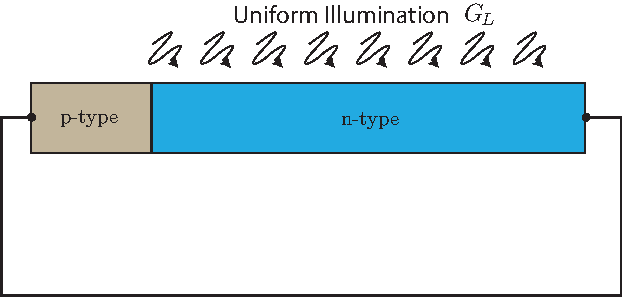
\includegraphics[width=.5\columnwidth]{pn_solar_cell}
\caption{A simple model for a solar cell ($PN$-junction) under equilibrium.  We assume the $N$-region is illuminated uniformly and calculate the minority carrier profile in the region to calculate the short circuit current.}
\label{fig:pn_solar_cell}
\end{figure}
%%%%%%%%%%%%%%%%%%%%%%%%%%%%%%%%%%%%%%%%%%%%
We are now in a position to derive the necessary parameters for a solar cell.   For simplicity, assume a very thin p$^+$ layer (no light illumination on the p$^+$ side) and optical carrier generation in the $N$-region.  Since there is no applied bias voltage on the pn junction, the boundary conditions at the edge of the depletion region is given by
    \begin{equation} 
        \Delta p(0) = 0  
    \end{equation}
On the other hand, if we travel far enough into the $N$-type region, we expect spatial variations to vanish and the number of excess holes should be directly proportional to the incoming light:
    \begin{equation} 
        \Delta p(\infty) = G_L \tau_p  
    \end{equation}
Using the general solution, and imposing boundary conditions, we have 
    \begin{equation} 
        \Delta p(x) = G_L \tau_p \left(1 - e^{-x/L_p} \right)   
    \end{equation}
 And the corresponding diffusion current is given by
    \begin{equation} 
        J_p(x) = - q D_p \frac{d \Delta p}{dx} = q \frac{D_p}{L_p}  \tau_p G_L  e^{-x/L_p}  
    \end{equation}
This means the short-circuit current is given by
    \begin{equation} 
        I_{sc} = A J_p(0) = A q L_p G_L 
    \end{equation}
Since in practice $G_L$ is not uniform, this result is only approximately true but it does give us some nice intuition for the important parameters.   In fact, the above equation is actually saying something very simple.  With reference to Fig.~\ref{fig:solar_cell_region}, only carriers generated within one diffusion length $L_p$ of the junction contribute to the current.  That's because optically generated minority carriers generated further don't actually end up reaching the junction, they recombine, and no net current flows.
%%%%%%%%%%%%%%%%%%%%%%%%%%%%%%%%%%%%%%%%%%%%
%                 FIGURE                   %
%%%%%%%%%%%%%%%%%%%%%%%%%%%%%%%%%%%%%%%%%%%%
\begin{figure}[tb]
\centering
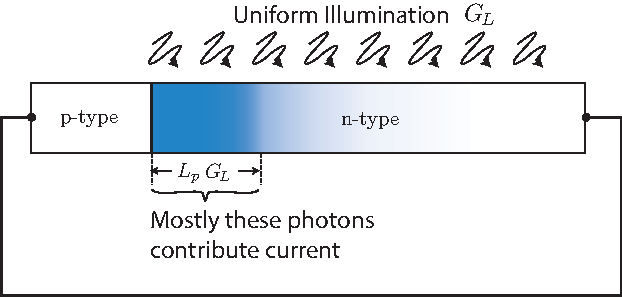
\includegraphics[width=.5\columnwidth]{solar_cell_region}
\caption{Due to recombination, only minority carriers generated within a diffusion length of the depletion region contribute significantly to the short circuit current.  Other generated minority carriers recombine and do not contribute net current.}
\label{fig:solar_cell_region}
\end{figure}
%%%%%%%%%%%%%%%%%%%%%%%%%%%%%%%%%%%%%%%%%%%%
%             SUBSECTION 6.7.5             %
%%%%%%%%%%%%%%%%%%%%%%%%%%%%%%%%%%%%%%%%%%%%
\subsection{Open Circuit Voltage}
Now we have an expression for the optically generated current and we can substitute it into the total diode current:
    \begin{equation} 
        I_D = \frac{A q n_i^2}{N_D} \frac{D_p}{L_p}  (e^{qV/kT} - 1) - A q L_p G_L 
    \end{equation}
Solving for the open-circuit voltage ($I_D = 0A$) and assuming the exponential dominates
    \begin{equation} 
        \frac{  n_i^2}{N_D} \frac{D_p}{L_p}  e^{qV_{oc} /kT}  =  L_p G_L 
    \end{equation}
which can be simplified to:
    \begin{equation} 
        V_{oc} = \frac{kT}{q} \ln \left( \frac{\tau_p G_L N_D}{n_i^2} \right) 
    \end{equation}
To generate a high open-circuit voltage, we need a large $\tau_p$, or very high quality semiconductors (low defect density).
%%%%%%%%%%%%%%%%%%%%%%%%%%%%%%%%%%%%%%%%%%%%
%             SUBSECTION 6.7.6             %
%%%%%%%%%%%%%%%%%%%%%%%%%%%%%%%%%%%%%%%%%%%%
\subsection{Light Emitting Diodes (LEDs)}
%%%%%%%%%%%%%%%%%%%%%%%%%%%%%%%%%%%%%%%%%%%%
%                 FIGURE                   %
%%%%%%%%%%%%%%%%%%%%%%%%%%%%%%%%%%%%%%%%%%%%
\begin{figure}[tb]
\centering
\includegraphics[width=.75\columnwidth]{led}
\caption{Light Emitting Diodes (LEDs) of various colors. [Wikipedia]}
\label{fig:led}
\end{figure}
%%%%%%%%%%%%%%%%%%%%%%%%%%%%%%%%%%%%%%%%%%%%
For LEDs (see Fig.~\ref{fig:led}), it's much more efficient to use a so-called ``direct band gap" material, defined below.  Common LEDs are InP and GaN.  Light is emitted when electrons and holes undergo radiative recombination (in silicon most of the energy is lost to phonons).  Let's see why by defigning a ``direct" and ``indirect" band gap.
%%%%%%%%%%%%%%%%%%%%%%%%%%%%%%%%%%%%%%%%%%%%
%              SUB-SUBSECTION              %
%%%%%%%%%%%%%%%%%%%%%%%%%%%%%%%%%%%%%%%%%%%%
\subsubsection*{Direct versus Indirect band gap Materials}
%%%%%%%%%%%%%%%%%%%%%%%%%%%%%%%%%%%%%%%%%%%%
%                 FIGURE                   %
%%%%%%%%%%%%%%%%%%%%%%%%%%%%%%%%%%%%%%%%%%%%
\begin{figure}[tb]
\centering
\begin{tabular}{cc}
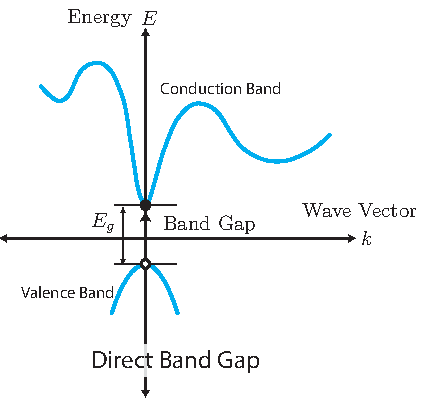
\includegraphics[width=.4\columnwidth]{bandgap_direct} & 
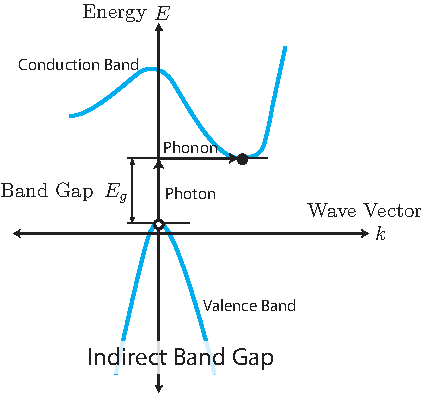
\includegraphics[width=.4\columnwidth]{bandgap_indirect}\\
(a) & (b)\\
\end{tabular}
\caption{(a) In a direct band gap material, such as $GaAs$, the peak of the valence band and the valley of the conduction band align in the momentum space, allowing a photon to be absorbed (or emitted) while conserving momentum.  (b)  In an indirect band gap material, such as silicon, absorption or emission of a photon requires the assistance of a phonon in order to conserve both energy and momentum.}
\label{fig:band gap_direct}
\end{figure}
%%%%%%%%%%%%%%%%%%%%%%%%%%%%%%%%%%%%%%%%%%%%
In this book we don't go into the details but it's important for now to realize that electrons have both energy $E$ and momentum $k$.  In a solid, the allowed energy-momentum states are dictated by quantum mechanics and plotted in an $E-k$ diagram, such as the ones shown in Fig.~\ref{fig:band gap_direct}.  In a direct band gap semiconductor, the bands overlap and an electron can absorb a photon \emph{directly} and become a conduction band electron with the same momentum.   In an indirect band gap, the top of the bands do not line up in $k$ space, so the assistance of a phonon is needed for optical generation, making the process less efficient and less likely to occur.  Silicon is an indirect band gap material while many compound semiconductors (group III + V elements together) are direct band gap materials.
%%%%%%%%%%%%%%%%%%%%%%%%%%%%%%%%%%%%%%%%%%%%
%                 FIGURE                   %
%%%%%%%%%%%%%%%%%%%%%%%%%%%%%%%%%%%%%%%%%%%%
\begin{figure}[tb]
\centering
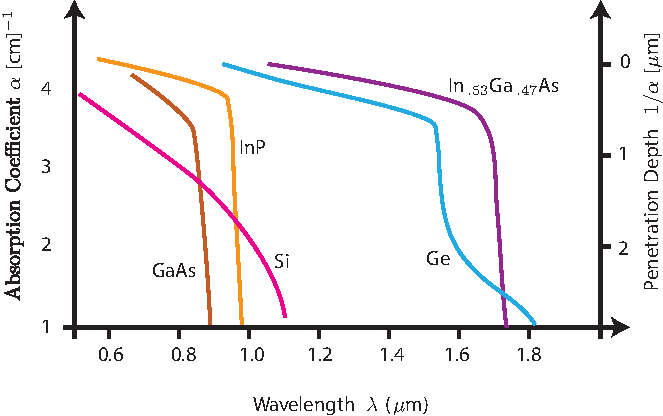
\includegraphics[width=.75\columnwidth]{semi_absorb_photon}
\caption{Qualitative plot of the absorption coefficient of various materials.  Notice that photons of a given wavelength can only be absorbed if they have sufficient energy to overcome the band gap.  This explains the sharp rise in the absorption coefficient for shorter wavelengths.} \label{fig:semi_absorb_photon}
\end{figure}
%%%%%%%%%%%%%%%%%%%%%%%%%%%%%%%%%%%%%%%%%%%%
It's also important to know how semiconductors absorb light.  A qualitative plot of photon absorption based on wavelength is shown in Fig.~\ref{fig:semi_absorb_photon}.  Light intensity is absorbed by a semi-conductor as long as the photon energy $E = h\nu = hc/\lambda $ is larger than the band gap.   Light intensity drops off exponentially $e^{-\alpha x}$ where $\alpha$ is the absorption coefficient.  
%%%%%%%%%%%%%%%%%%%%%%%%%%%%%%%%%%%%%%%%%%%%
%                 FIGURE                   %
%%%%%%%%%%%%%%%%%%%%%%%%%%%%%%%%%%%%%%%%%%%%
\begin{figure}[tb]
\centering
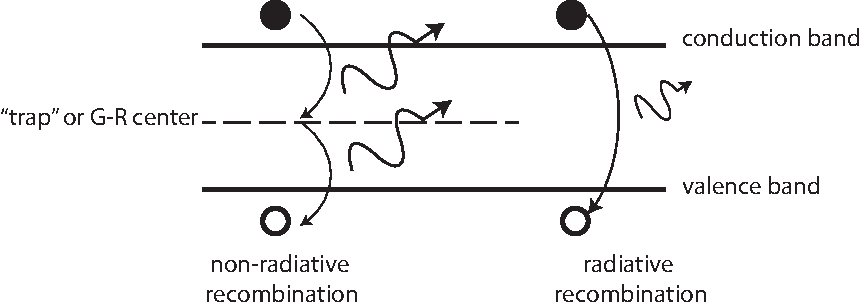
\includegraphics[width=.75\columnwidth]{rad_vs_nonrad_reco}
\caption{In an indirect band gap material, such as silicon, most recombination occurs through a trap (crystal defect or impurity) and generates phonons (left).  In a direct band gap material, recombination leads to optical photons (right).}
\label{fig:rad_vs_nonrad_reco}
\end{figure}
%%%%%%%%%%%%%%%%%%%%%%%%%%%%%%%%%%%%%%%%%%%%
For the generation of photon, a direct band gap material is preferred.  Direct recombination is efficient as $k$ is conserved (momentum).  In an indirect band gap, direct recombination is rare as $k$ is not conserved.  Most recombination is trap assisted and does not produce optical photons (as shown in Fig.~\ref{fig:rad_vs_nonrad_reco}).  This is the case with silicon and this why most LEDs are not made with silicon. For efficient light generation, we prefer a direct band gap, and many III-V compound semiconductors have this property.  Compound semiconductors are made with a mixture of group III and group V atoms, and have similar properties as semiconductors made of group III atoms.
%%%%%%%%%%%%%%%%%%%%%%%%%%%%%%%%%%%%%%%%%%%%
%             SUBSECTION 6.7.7             %
%%%%%%%%%%%%%%%%%%%%%%%%%%%%%%%%%%%%%%%%%%%%
\subsection{LED Materials and Structure}
%%%%%%%%%%%%%%%%%%%%%%%%%%%%%%%%%%%%%%%%%%%%
%                 FIGURE                   %
%%%%%%%%%%%%%%%%%%%%%%%%%%%%%%%%%%%%%%%%%%%%
\begin{figure}[tb]
\centering
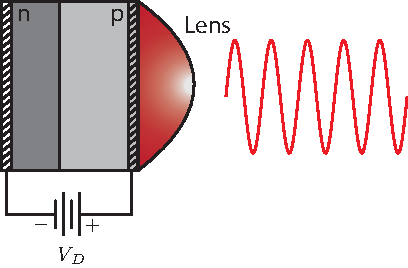
\includegraphics[width=.35\columnwidth]{led_struct}
\caption{An LED is simply a forward biased pn junction made with a direct band gap material and constructed to collect photons.  A lens is often used to collimate the light to maximize the intensity.  Compare with Fig.~\ref{fig:led}.}
\label{fig:led_struct}
\end{figure}
%%%%%%%%%%%%%%%%%%%%%%%%%%%%%%%%%%%%%%%%%%%%
The structure of an LED $PN$-junction diode is shown in Fig.~\ref{fig:led_struct}.  A lens is used to capture photons traveling in different directions and to collimate the beam of light for higher intensity.    The direct band gap material is forward biased and the current flow results in minority carrier injection, which results in (mostly) radiative recombination.  To avoid re-absorbing the photons, the materials and structure are carefully designed to emit light. 
%%%%%%%%%%%%%%%%%%%%%%%%%%%%%%%%%%%%%%%%%%%%
Each radiative recombination event generates a photon with energy of the band gap, which allows us to find the wavelength of the photon by equating the energy of a photon $h \nu$ (frequency $\nu$) with the band gap energy:
    \begin{equation} 
        E_g = h \nu = h c / \lambda_{\text{LED}} 
    \end{equation}
Solving for the wavelength of the emitted photon, we have:
    \begin{equation} 
        \lambda_{\text{LED}} = \frac{hc}{E_g} = \frac{1.24}{E_g \text{(eV)}}
    \end{equation}
where we have used common units of eV since most band gaps are also reported in this energy unit.  In Table~\ref{tab:rainbow}, we calculate the wavelength based on the reported band gap of several commonly used compound semiconductors.  These values can be found in references and on the web, although there is some variation in the literature.
    \begin{table}[htbp]
    \begin{center}
      \caption{Commonly Used Compound Semiconductors}
        \begin{tabular}{cccc}
        \toprule
        & $E_g$ (eV) & $\lambda$ ($\mu$m) & \textbf{Color} \\
        \midrule
        \rowcolor[rgb]{ .851,  .851,  .851} InAs  & 0.35  & 3.51  & infrared \\
        InN   & 0.65  & 1.91  & infrafed \\
        \rowcolor[rgb]{ .851,  .851,  .851} InP   & 1.34  & 0.92  & infrafed \\
        GaAs  & 1.43  & 0.87  & Red \\
        \rowcolor[rgb]{ .851,  .851,  .851} GaP   & 2.26  & 0.55  & Yellow \\
        AlP   & 2.45  & 0.51  & Green \\
        \rowcolor[rgb]{ .851,  .851,  .851} GaN   & 3.40  & 0.37  & Blue \\
        AlN   & 6.20  & 0.20  & UV \\
        \bottomrule
        \end{tabular}
      \label{tab:rainbow}
    \end{center}
    \end{table}
%%%%%%%%%%%%%%%%%%%%%%%%%%%%%%%%%%%%%%%%%%%%%%%%%%%%%%%%%%%%%%%%%%%%%%%%%%%%%%%%%%%%%%%%
%%%%%%%%%%%%%%%%%%%%%%%%%%%%%%%%%%%%%%%%%%%%%%%%%%%%%%%%%%%%%%%%%%%%%%%%%%%%%%%%%%%%%%%%
%                                   SECTION 6.8                                        %
%%%%%%%%%%%%%%%%%%%%%%%%%%%%%%%%%%%%%%%%%%%%%%%%%%%%%%%%%%%%%%%%%%%%%%%%%%%%%%%%%%%%%%%%
%%%%%%%%%%%%%%%%%%%%%%%%%%%%%%%%%%%%%%%%%%%%%%%%%%%%%%%%%%%%%%%%%%%%%%%%%%%%%%%%%%%%%%%%
\section{References}
Much of this material comes from teaching EE 105 at UC Berkeley for several years.  The notes have benefited greatly from Pierret (\emph{Semiconductor Fundamentals: Volume I}), and most recently from Chenming Hu (\emph{Modern Semiconductor Devices for Integrated Circuits}).
